\documentclass{ctexart}
\usepackage{amsmath}
\usepackage{float}
\usepackage{graphicx}
\usepackage[a4paper,left=25mm,right=25mm,top=31mm,bottom=31mm]{geometry}
\pagestyle{plain}
\graphicspath{{./images}}


\begin{document}

\begin{center}
    \LARGE \textbf{企业实习\;第五周实习报告}\\
    \vspace{10pt}
    \normalsize 小米自动驾驶与机器人部\;\;陈子林
\end{center}

\section{本周工作主要内容}

本周为小米实习第一周 (7.21--7.25),主要工作内容如下:

\begin{enumerate}
    \item 学习阅读机械臂相关文献,了解DH参数及相关计算问题,掌握齐次变换矩阵、旋转矩阵、欧拉角等数学工具。
    \item 利用C++开发相关算法,计算机械臂正运动学,为后续工作做各种准备工作(如构建相关class,部分数学工具的编写)。
    \item 对机械臂进行工作空间分析,选择合理的工作范围,并进行moveL、moveJ等函数进行设计与测试,如图\ref{demo}所示。
    \begin{figure}[H]
        \centering
        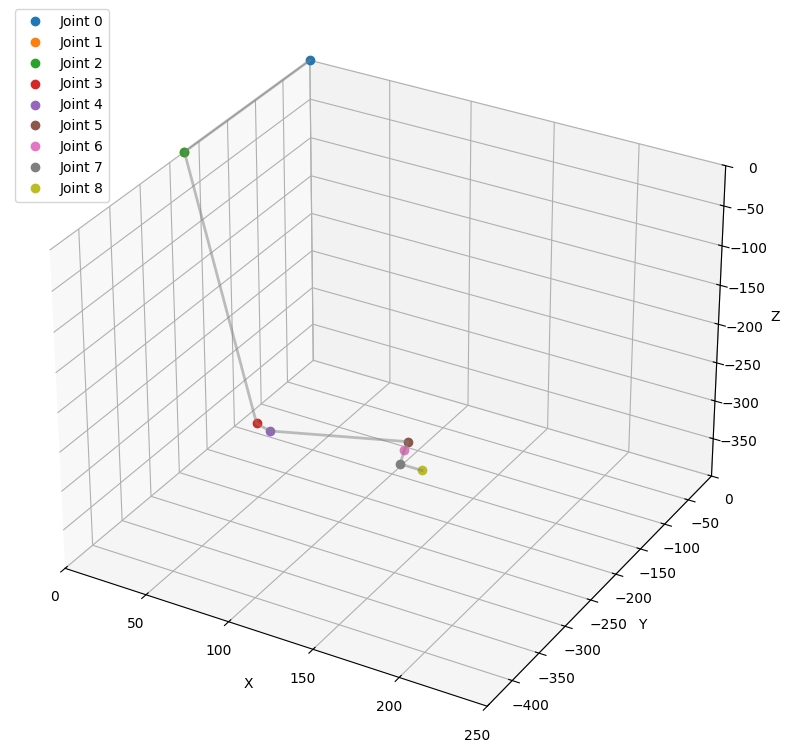
\includegraphics[width = 0.4\textwidth]{figure2.jpg}
        \caption{机械臂示意图}\label{demo}
    \end{figure}
    \item 构建迭代器求解机械臂逆运动学,得到指定末端位姿下的关节角,如图\ref{joint}所示。
    \begin{figure}[H]
        \centering
        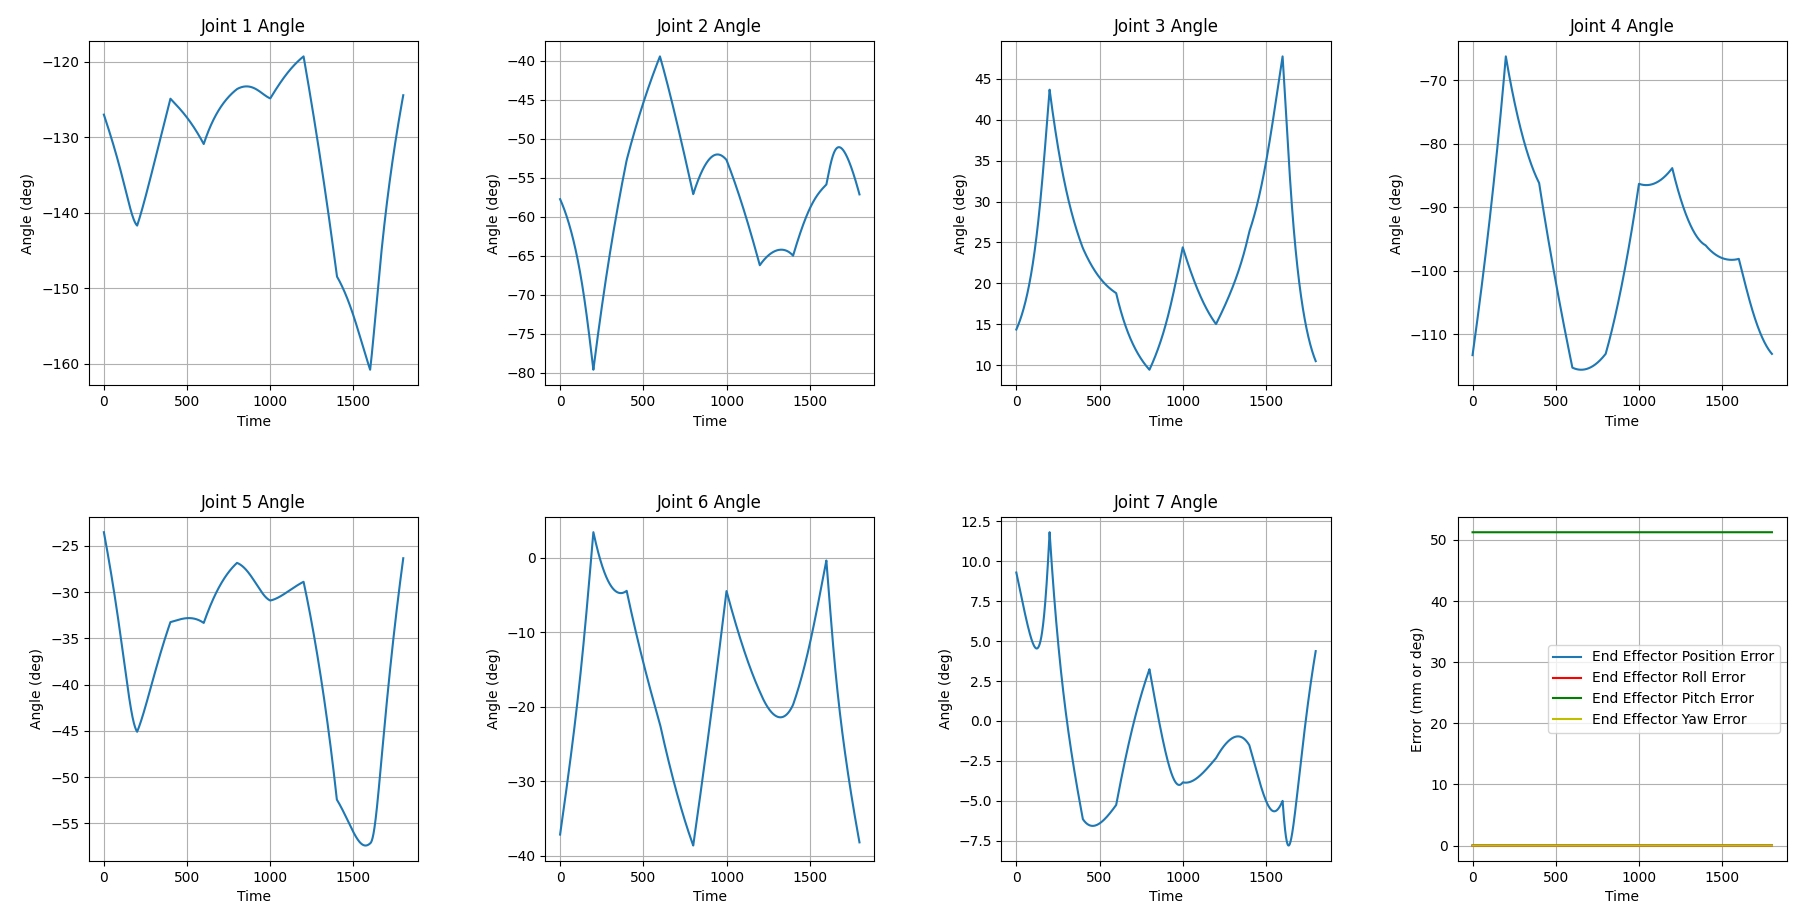
\includegraphics[width = 0.7\textwidth]{figure1.jpg}
        \caption{机械臂关节角度及末端误差}\label{joint}
    \end{figure}
    \item 阅读国标相关文件(GBT 12642--2013/ISO 9283:1998),为后续机械臂开展国标验证做好准备。
    
\end{enumerate}

\section{后续工作计划}

针对目前实习目标和工作进度,下一阶段计划如下:

\begin{enumerate}
    \item 学习滤波器算法,消除轨迹规划后的毛刺和明显错误的转折点,使得关节角度平滑变化。
    \item 参观实体样机,选择合适工作空间规划运动轨迹,进行国标测试前的准备工作。
    \item 编写readme等相关技术文档,为后续进一步开发或后期交接工作做好准备。
    \item 调试相关接口,为后续与硬件、仿真器联动进行HIL测试做好相应准备。
\end{enumerate}

\end{document}